\section[Beam Current Measurement]{Beam Current Measurement
\footnote{Authors: D.Higinbotham \email{doug@jlab.org} with thanks to A.Saha$^{Deceased}$}
}

The Beam Current Monitor (BCM) is designed for stable, low noise, non-intercepting 
beam current measurements. It consists of an Unser monitor, two rf cavities, 
the electronics and a data acquisition system. The cavities and the Unser monitor 
are enclosed in a box to improve magnetic shielding and temperature stabilization.
The box is located 25 m upstream of the target. You can recognize it as a grey 
object on the stands, about 2 m downstream from where the beam enters the 
hall. 

The DC 200 down-converters and the Unser front end electronics are located in Hall 
A. The temperature controller, the Unser back end electronics and its calibration 
current source, cavity's RF unit (housing the RMS-to-DC converter board) and all 
multi-meters, VME crate and computers are located in Hall A control room.

\infolevone{
\subsection{ System Layout}

The schematic diagram of the BCM system is presented in
Fig.~\ref{fig:halla_bcm}.
\begin{figure}[htp]
\begin{center}
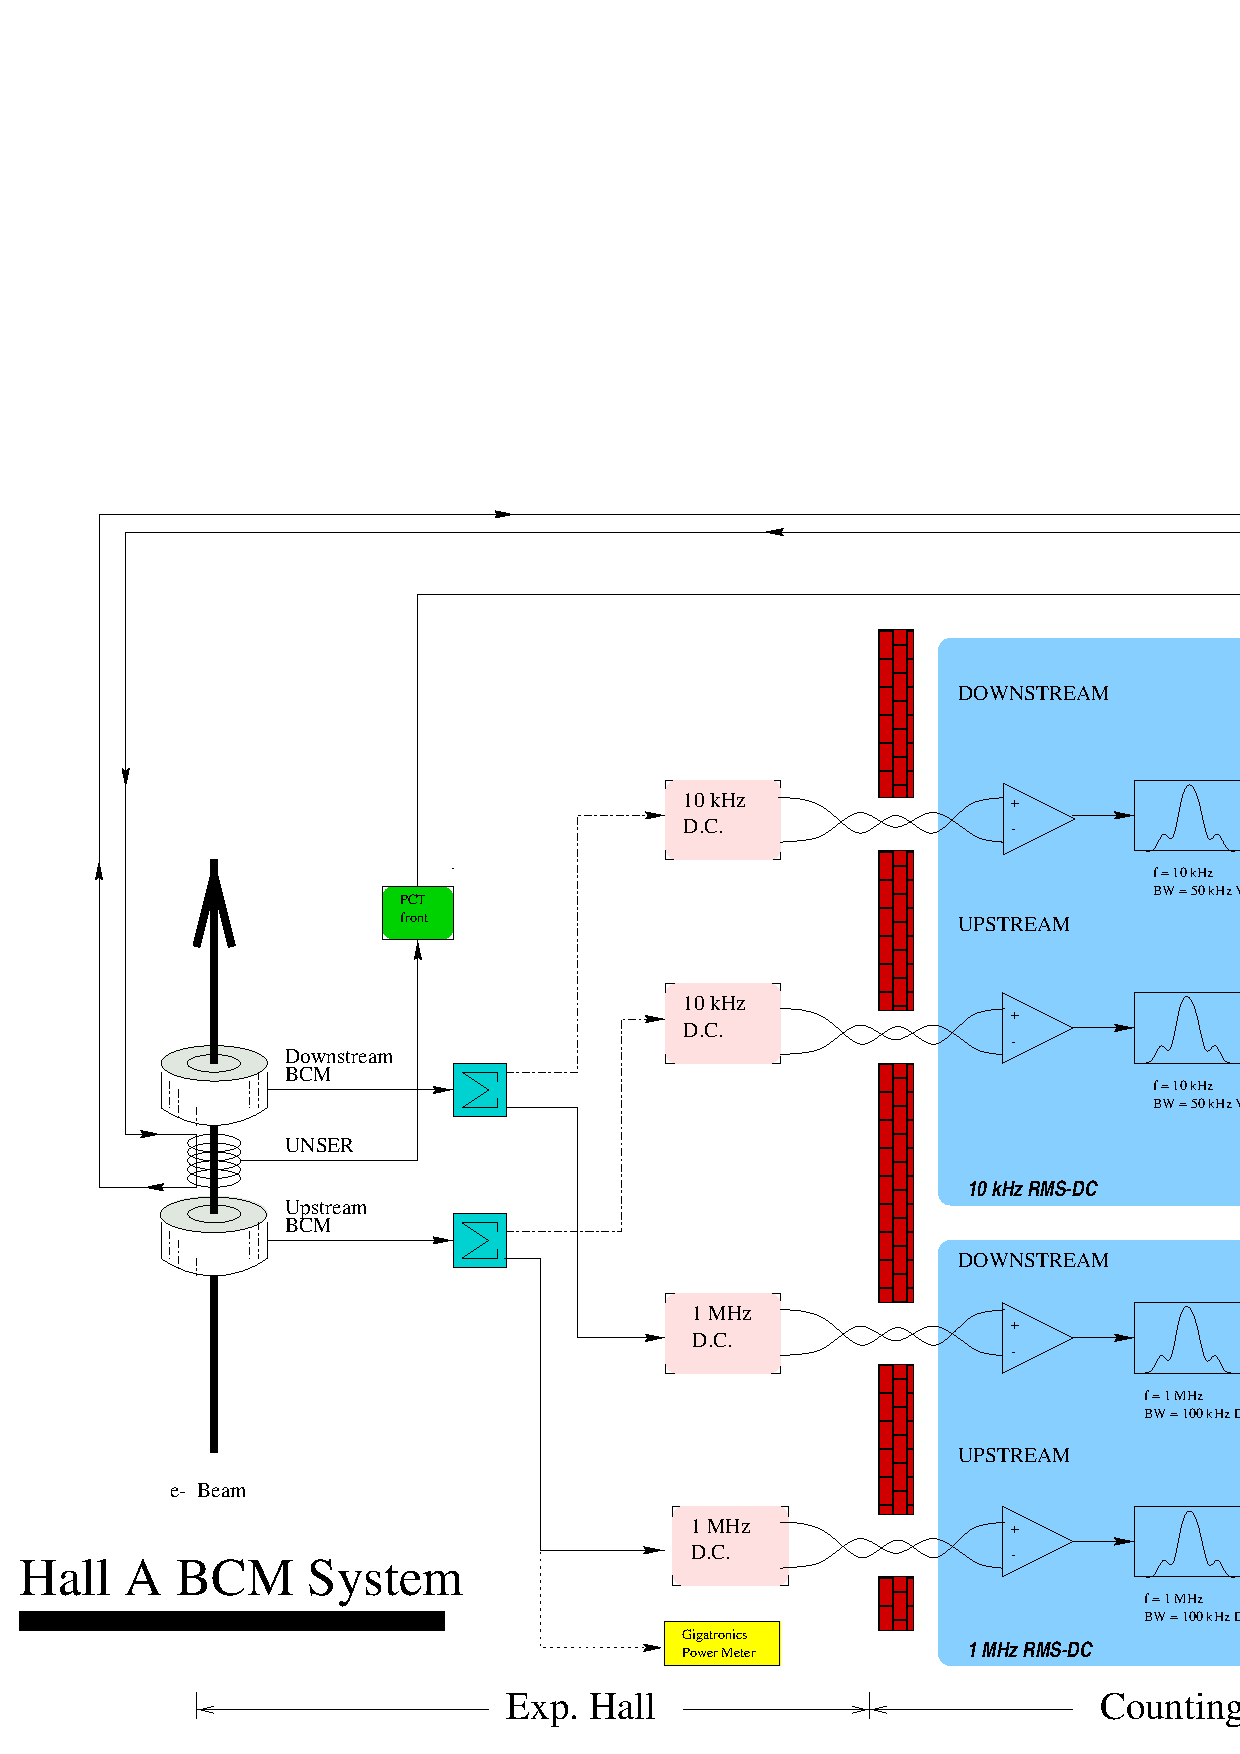
\includegraphics[angle=0,width=0.9\textwidth,clip]{habcm_r}
{\linespread{1.}
\caption[Beam Current Measurement: Schematic]{Schematic of the Hall A beam
current measurement system.}
\label{fig:halla_bcm}}
\end{center}
\end{figure}

The Unser monitor is a Parametric Current Transformer designed for non-destructive 
beam current measurement and providing an absolute reference. The monitor is 
calibrated by passing a known current through a wire inside the beam pipe and has a 
nominal output of 4 mV/$\mu $A. It requires extensive magnetic shielding and 
temperature stabilization to reduce noise and zero drift. As the Unser monitor's 
output signal drifts significantly on a time scale of several minutes, it cannot be 
used to continuously monitor the beam current. However, this drift is measured 
during the calibration runs (by taking a zero current reading) and removed in 
calibrating the cavities.  The more stable cavities are then used to determine the 
beam current and charge for each run. We also use the OLO2 Cavity Monitor and the 
Faraday Cup 2 at the Injector section to provide an absolute reference during 
calibration runs.

The two resonant rf cavity monitors on either side of the Unser Monitor are 
stainless steel cylindrical high Q ($\sim 3000$) waveguides which are tuned to the 
frequency of the beam (1.497 GHz) resulting in voltage levels at their   outputs 
which are proportional to the beam current. Each of the rf output signals from the 
two cavities are split into two parts. One part of the signal is  converted to 10 
kHz signals (by the ``downconverters'') and fed into an RMS-to-DC converter board 
consisting of a 50 kHz bandpass filter to  eliminate noise, amplified and split to 
two sets of outputs, which after further processing are recorded in the data 
stream. These two paths to the data stream (leading to the sampled and integrated
data ) will now be described. (The other part of the split signal is downconverted 
to 1 MHz signals and represents the old system (pre Jan 99). Only the HAPPEX 
collaboration presently uses these signals.)

For the sampled (or EPICS~\cite{EPICSwww} or Slow) data, one of the amplifier outputs is sent to a 
high precision digital AC voltmeter (HP 3458A). Each second this device provides 
a digital output which represents the  RMS average of the input signal during that 
second.  The resulting number is  proportional to the beam charge accumulated 
during the corresponding second (or, equivalently, the average  beam current  for 
that second). Signals from both cavity's multi-meters, as well as from the 
multi-meter connected to the Unser, are transported through GPIB ports to the HAC 
computer where they are recorded every 1 to 2 seconds via the data-logging process 
which is described in the calibration procedure. They are also sent through EPICS 
to CODA and the data stream where they are recorded at  quasi-regular intervals, 
typically every two to five  seconds.

For the integrated (or VTOF or Fast) data, the other amplifier output is sent to an 
RMS-to-DC converter which   produces  an analog DC  voltage  level. This level 
drives a Voltage-To-Frequency (VTOF) converter whose output frequency is  
proportional to the  input DC voltage level. These signals are then fed to Fastbus  
scalers and are finally injected into the data stream along  with the other scaler 
information.  These scalers simply accumulate during  the run, resulting  in a 
number which is proportional to the time integrated voltage level and therefore 
more accurately represents the true integral of the current and hence the total 
beam charge. The regular RMS to DC output is linear for currents
from about 5 $\mu$A to somewhere well above 200 $\mu$A.
 Since it is non-linear at the lower 
currents, we have introduced a set of amplifiers with differing gains (x3 and x10) 
allowing the non-linear region to be extended to lower currents at the expense of 
saturation at the very high currents. Hence there are 3 signals coming 
from each BCM (Upx1, Upx3, Upx10, Dnx1, Dnx3, Dnx10). All 6 signals are fed 
to scaler inputs of each spectrometer (E-arm and H-arm) . Hence we have a 
redundancy of 12 scaler outputs for determining the charge during a run. During 
calibration runs we calibrate each of these scaler outputs.   
}

\begin{safetyen}{10}{10}
\subsection{ Authorized Personnel}
\end{safetyen}

All Hall A members are authorized to take BCM calibration data using the Standard 
Non-Invasive Hall A BCM Calibration Procedure. The extended calibration procedures 
involving the Faraday Cup 2 and the OLO2 monitor at the Injector are presently 
performed by A. Saha. 

\vskip 0.2cm

The Accelerator EES group performs the maintenance of the BCM monitors. These 
include:

\begin{tabular}{l l}
1. The Unser calibration. & Every 3 months \\
2. Resonant Cavities Tuning. & Every Downtime \\
3. Multi-meters Autocalibration. & Every Downtime \\
4. Connectors Cleaning. &  Every year \\
5. Unser Keithley Current Source. & Calibration Yearly \\
6. Digital Multi-meters HP3458A and HP 34401A. & Calibration Yearly\\   
\end{tabular}

System Contacts are shown in Table~\ref{tab:BCM:personnel}.
\begin{namestab}{tab:BCM:personnel}{BCM: authorized personnel}{%
   Beam Current Monitor: authorized personnel}
  \ArunSaha{\em Contact}
  \JohnMusson{Accel. expert}
\end{namestab}
%Jean-Claude Denard -x 7555




